% 按固定来源第7扫描页可见点线关系重绘；仅作示意，不按比例，也不增加垂直标记。
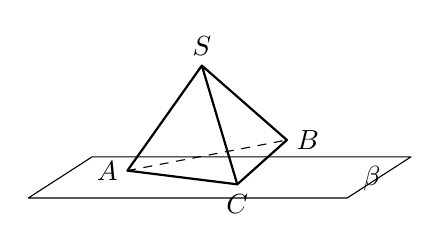
\begin{tikzpicture}[x=0.9cm,y=0.58cm,line cap=round,line join=round]
  \coordinate (P1) at (-2.4,-0.55);
  \coordinate (P2) at (2.1,-0.55);
  \coordinate (P3) at (3.0,0.35);
  \coordinate (P4) at (-1.5,0.35);
  \coordinate (A) at (-1.0,0.05);
  \coordinate (B) at (1.25,0.72);
  \coordinate (C) at (0.55,-0.25);
  \coordinate (S) at (0.05,2.35);
  \draw[thin] (P1)--(P2)--(P3)--(P4)--cycle;
  \node at (2.45,-0.12) {$\beta$};
  \draw[thick] (A)--(C)--(B);
  \draw[dashed] (A)--(B);
  \draw[thick] (S)--(A) (S)--(B) (S)--(C);
  \node[left] at (A) {$A$};
  \node[right] at (B) {$B$};
  \node[below] at (C) {$C$};
  \node[above] at (S) {$S$};
\end{tikzpicture}
